\section{GPU 编程}
在过去的几十年里,图形处理单元 (GPU) 已经从能够在屏幕上绘制图像的专用硬件设备发展为能够执行复杂并行Kernel的通用设备。 
如今,几乎每台计算机都在传统 CPU 旁边配备了 GPU,并且可以通过将部分并行算法从 CPU 卸载到 GPU 来加速许多程序。

在本章中,我们将描述典型 GPU 的工作原理、GPU 软件和硬件如何执行 SYCL 应用程序,
以及在为 GPU 编写和优化并行Kernel时要记住的提示和技术。

\subsection{性能注意事项}
与任何处理器类型一样,GPU 因供应商而异,甚至因产品一代而异; 
因此,一种设备的最佳实践可能并不适用于其他设备的最佳实践。 
本章中的建议可能会让许多 GPU 现在和将来受益,但是……

\begin{remark}
	要实现特定 GPU 的最佳性能,请务必查阅 GPU 供应商的文档!
\end{remark}

本章末尾提供了来自许多 GPU 供应商的文档链接。

\subsection{GPU 的工作原理}
本节介绍典型 GPU 的工作原理以及 GPU 与其他加速器类型的不同之处。

\subsubsection{GPU 构建模块}
\begin{figure}[H]
	\centering
	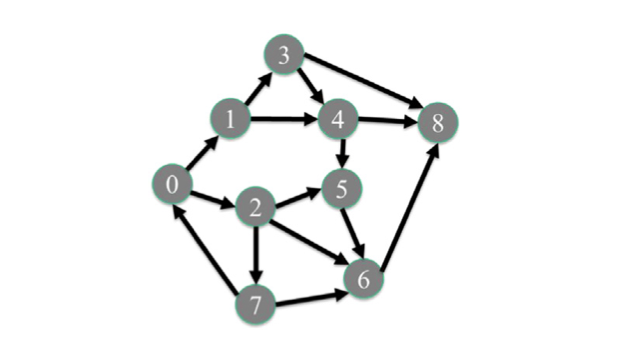
\includegraphics[width=0.9\textwidth]{figs/F15.1.png}
	\caption{\textit{典型的 GPU 构建块 — 无法扩展! }}
\end{figure}

图 15-1 显示了一个非常简化的 GPU,由三个高级构建块组成:

\begin{enumerate}
	\item \textbf{执行资源} :GPU的执行资源是执行计算工作的处理器。 
不同的 GPU 供应商对其执行资源使用不同的名称,但所有现代 GPU 都由多个可编程处理器组成。 
处理器可以是异构的并且专门用于特定任务,例如变换顶点和着色像素,或者它们可以是同构的并且可互换。 
大多数现代 GPU 的处理器都是同质且可互换的。

	\item \textbf{固定函数}:GPU固定函数是比执行资源可编程性更差的硬件单元,专门用于单个任务。 
当 GPU 用于图形时,图形管道的许多部分(例如光栅化或光线追踪)都是使用固定函数执行的,以提高功效和性能。 
当GPU用于数据并行计算时,固定函数可以用于诸如工作负载调度、纹理采样和依赖性跟踪等任务。

	\item \textbf{高速缓存和内存}:与其他处理器类型一样,GPU 经常具有高速缓存来存储执行资源访问的数据。 
GPU 缓存可以是隐式的,在这种情况下,它们不需要程序员执行任何操作,或者可以是显式暂存器存储器,
在这种情况下,程序员必须在使用数据之前有目的地将数据移动到缓存中。 
许多 GPU 还拥有大量内存,可以快速访问执行资源所使用的数据。
\end{enumerate}

\subsubsection{更简单的处理器(但数量更多)}
传统上,在执行图形操作时,GPU 会处理大量数据。 
例如,典型的游戏帧或渲染工作负载涉及数千个顶点,每帧产生数百万个像素。 
为了保持交互式帧速率,必须尽快处理这些大批量数据。

\begin{figure}[H]
	\centering
	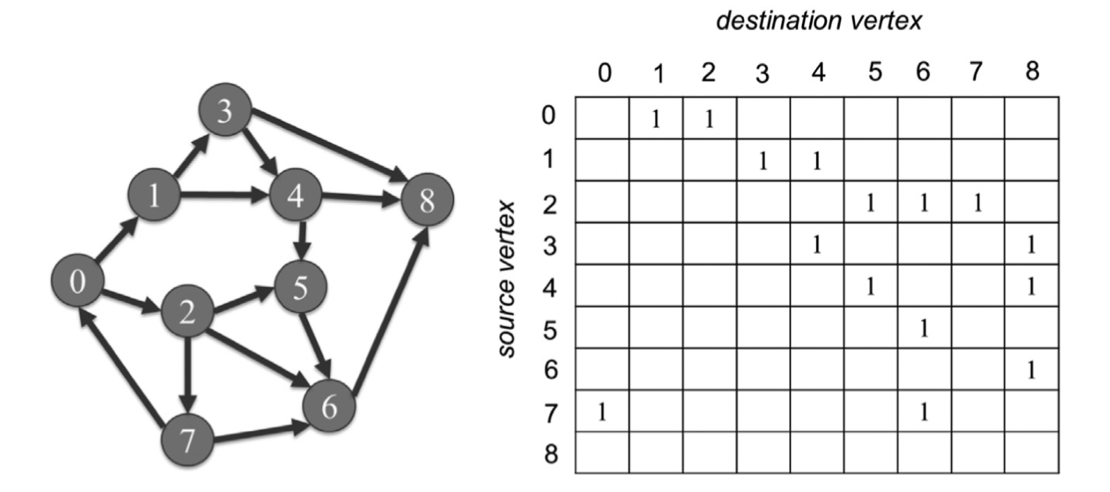
\includegraphics[width=0.9\textwidth]{figs/F15.2.png}
	\caption{\textit{GPU 处理器更简单,但数量更多 }}
\end{figure}

典型的 GPU 设计权衡是消除形成加速单线程性能的执行资源的处理器的功能,并利用这些节省来构建额外的处理器,
如图 15-2 所示。 例如,GPU 处理器可能不包括其他类型处理器使用的复杂的乱序执行功能或分支预测逻辑。 
由于这些权衡,单个数据元素在 GPU 上的处理速度可能比在另一个处理器上的速度慢,
但处理器数量较多使 GPU 能够快速高效地处理许多数据元素。

为了在执行Kernel时利用这种权衡,为 GPU 提供足够大范围的数据元素进行处理非常重要。 
为了证明卸载大量数据的重要性,请考虑我们在整本书中开发和修改的矩阵乘法Kernel。

\begin{remark}[关于矩阵乘法的提醒]
	在本书中,矩阵乘法Kernel用于演示Kernel的变化或其调度方式如何影响性能。
	尽管使用本章中描述的技术显著提高了矩阵乘法性能,但矩阵乘法是一项非常重要且常见的操作,
	以至于许多硬件(GPU、CPU、FPGA、DSP 等)供应商已经实现了许多例程(包括矩阵乘法)的高度调整版本。
	这些供应商投入了大量的时间和精力来实现和验证特定设备的功能,
	在某些情况下,可能会使用在标准Kernel中难以或不可能使用的功能或技术。

使用供应商提供的库!

当供应商提供函数的库实现时,使用它几乎总是有益的,而不是将函数重新实现为Kernel!
oneMKL 项目(oneAPI 的一部分)提出了一些接口,
这些接口将调用 intel 的 MKL 用于 intel,cuBLas 用于 NVIDIA,hipBlas 用于 AMD。如果此类接口可用,
它们可能会使事情变得更容易。否则,我们需要做自己的工作,以确保我们为目标硬件使用最好的库。
\end{remark}

通过将矩阵乘法Kernel作为单个任务提交到队列中,可以在 GPU 上轻松执行。 
该矩阵乘法Kernel的主体看起来与主机 CPU 上执行的函数完全相同,如图 15-3 所示。

\begin{figure}[H]
	\centering
	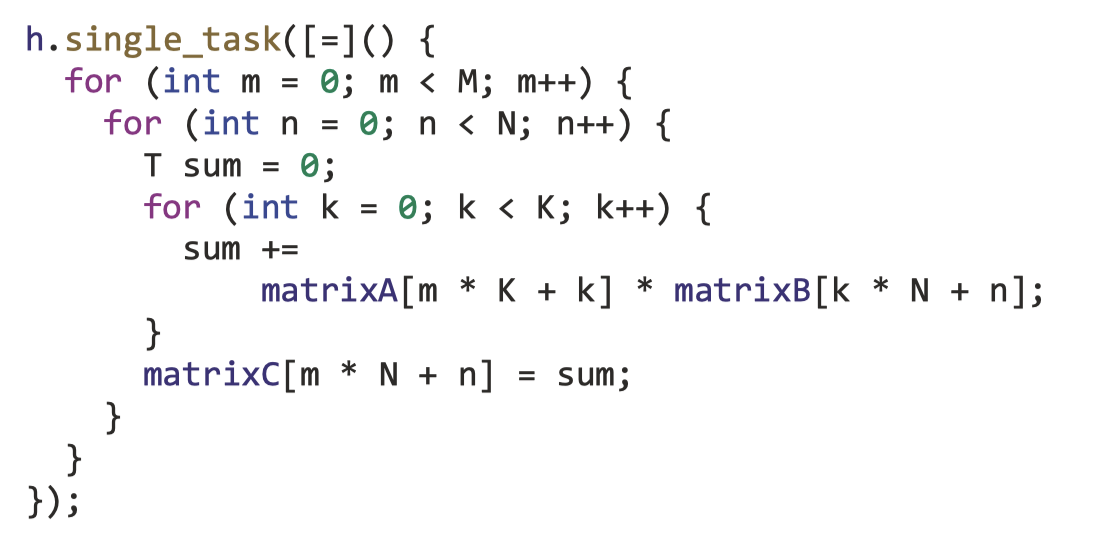
\includegraphics[width=0.9\textwidth]{figs/F15.3.png}
	\caption{\textit{单任务矩阵乘法看起来很像 CPU 主机代码 }}
\end{figure}

如果我们尝试在 CPU 上执行该Kernel,它的性能可能还不错,但不是很好,
因为预计它不会利用 CPU 的任何并行功能,但对于小矩阵大小来说可能足够好。 
然而,如图 15-4 所示,如果我们尝试在 GPU 上执行该Kernel,它的性能可能会很差,因为单个任务只会使用单个 GPU 处理器。

\begin{figure}[H]
	\centering
	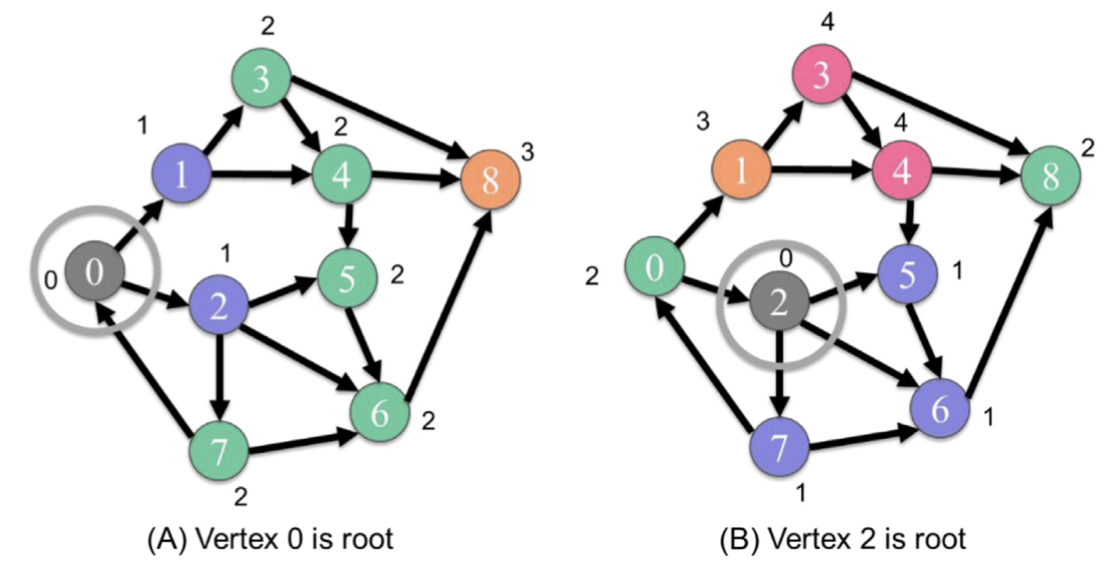
\includegraphics[width=0.9\textwidth]{figs/F15.4.png}
	\caption{\textit{GPU 上的单任务Kernel会使许多执行资源处于空闲状态 }}
\end{figure}

\paragraph{表达并行性}

为了提高该Kernel对于 CPU 和 GPU 的性能,
我们可以通过将其中一个循环转换为 parallel\_for 来提交一系列数据元素进行并行处理。 
对于矩阵乘法Kernel,我们可以选择提交代表两个最外层循环之一的一系列数据元素。 
在图 15-5 中,我们选择并行处理结果矩阵的行。

\begin{figure}[H]
	\centering
	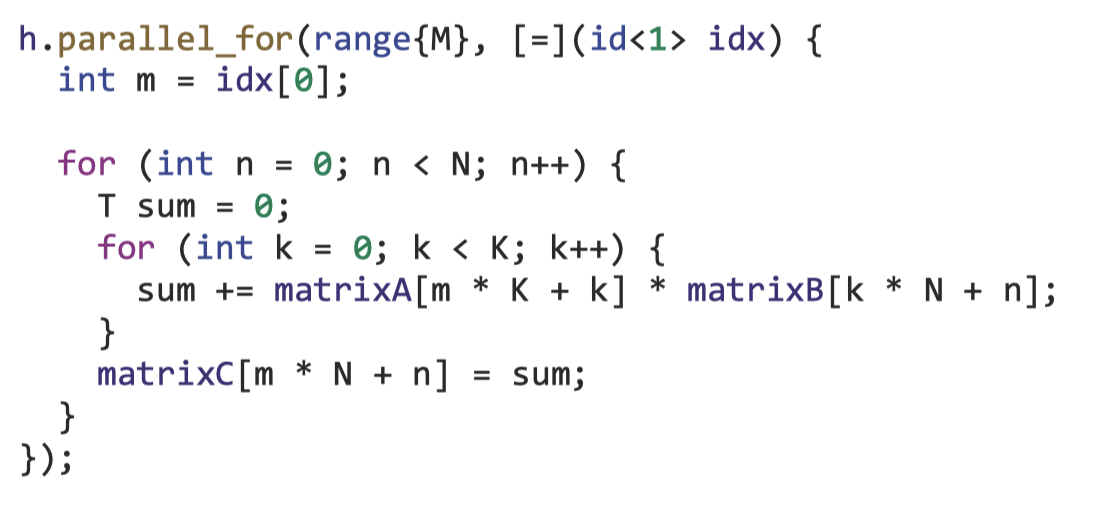
\includegraphics[width=0.9\textwidth]{figs/F15.5.png}
	\caption{\textit{某种平行矩阵乘法 }}
\end{figure}

\begin{remark}[选择如何并行化]
选择要并行化的维度是针对 GPU 和其他设备类型调整应用程序的一种非常重要的方法。
本章的后续部分将介绍为什么在一个维度中并行化可能比在另一个维度中并行化效果更好的一些原因。
\end{remark}

\begin{figure}[H]
	\centering
	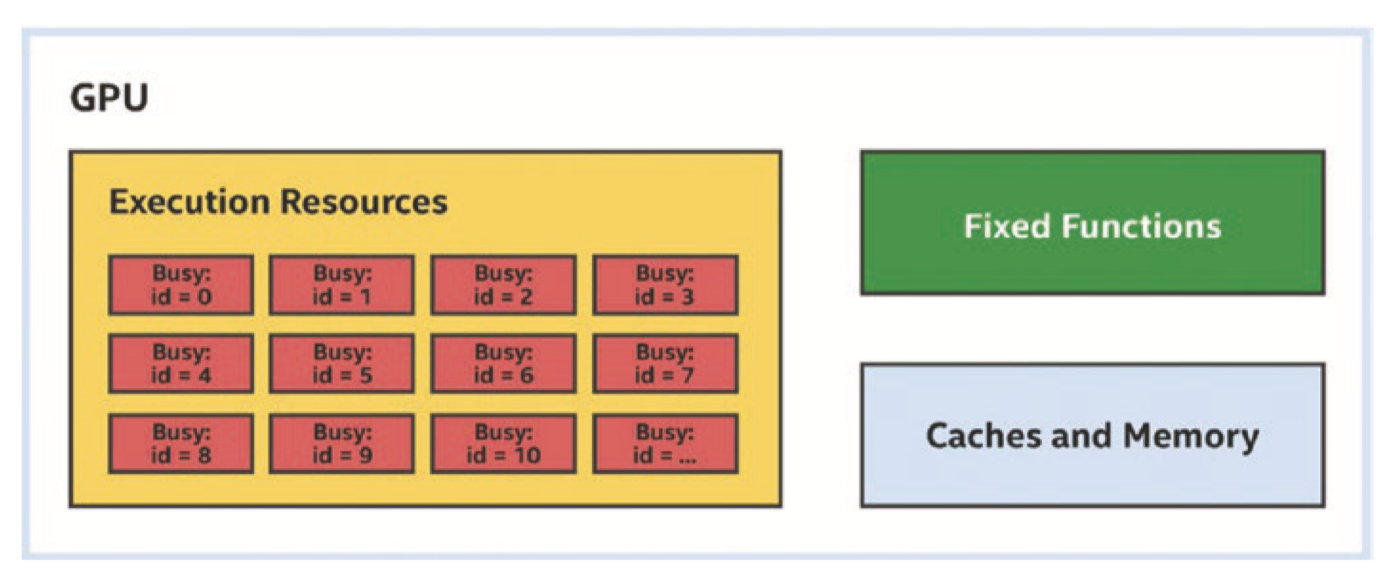
\includegraphics[width=0.9\textwidth]{figs/F15.6.png}
	\caption{\textit{某种程度上并行的Kernel使更多的处理器资源保持忙碌 }}
\end{figure}

尽管有点并行的Kernel与单任务Kernel非常相似,但它在 CPU 上运行得更好,在 GPU 上运行得更好。 
如图 15-6 所示,parallel\_for 使代表结果矩阵行的Work-Items能够在多个处理器资源上并行处理,
因此所有执行资源都保持忙碌状态。

请注意,未指定行分区和分配给不同处理器资源的确切方式,从而使实现能够灵活地选择如何最好地在设备上执行Kernel。 
例如,实现可以选择在同一处理器上执行连续的行以获得局部性优势,而不是在处理器上执行单独的行。

\paragraph{表达更多的并行性}

\begin{figure}[H]
	\centering
	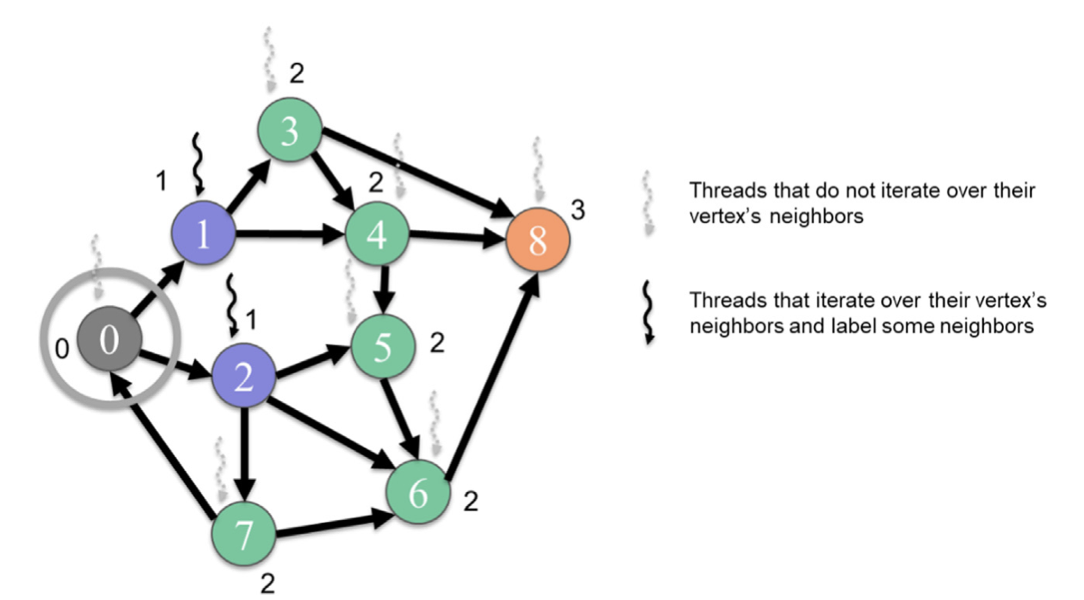
\includegraphics[width=0.9\textwidth]{figs/F15.7.png}
	\caption{\textit{更多并行矩阵乘法 }}
\end{figure}

通过选择并行处理两个外部循环,我们可以进一步并行化矩阵乘法Kernel。 
因为 parallel\_for 可以在最多三个维度上表达并行循环,所以这很简单,如图 15-7 所示。 
在图15-7中,请注意传递给parallel\_for的范围和表示并行执行空间中索引的项现在都是二维的。

当在 GPU 上运行时,暴露额外的并行性可能会提高矩阵乘法Kernel的性能。 
即使矩阵行数超过 GPU 处理器的数量,情况也可能如此。 接下来的几节将描述出现这种情况的可能原因。

\subsubsection{简化的控制逻辑(SIMD 指令)}
许多 GPU 处理器利用大多数数据元素倾向于通过Kernel采用相同的控制流路径这一事实来优化控制逻辑。 
例如,在矩阵乘法Kernel中,每个数据元素执行最内层循环的次数相同,因为循环边界是不变的。

当数据元素通过Kernel采用相同的控制流路径时,
处理器可以通过在多个数据元素之间共享控制逻辑并将它们作为一组执行来降低管理指令流的成本。 
实现此目的的一种方法是实现单指令、多数据或 SIMD 指令集,其中单指令同时处理多个数据元素。

\begin{remark}[线程 VS.指令流]
在许多并行编程上下文和 GPU 文献中,术语“线程”用于表示“指令流”。
在这些上下文中,“线程”不同于传统的操作系统线程,通常更轻量级。
然而,情况并非总是如此,在某些情况下,“线程”被用来描述完全不同的东西。

由于术语“线程”过载且容易被误解,即使在不同的 GPU 供应商之间也是如此,因此本章改用术语“指令流”。
\end{remark}

\begin{figure}[H]
	\centering
	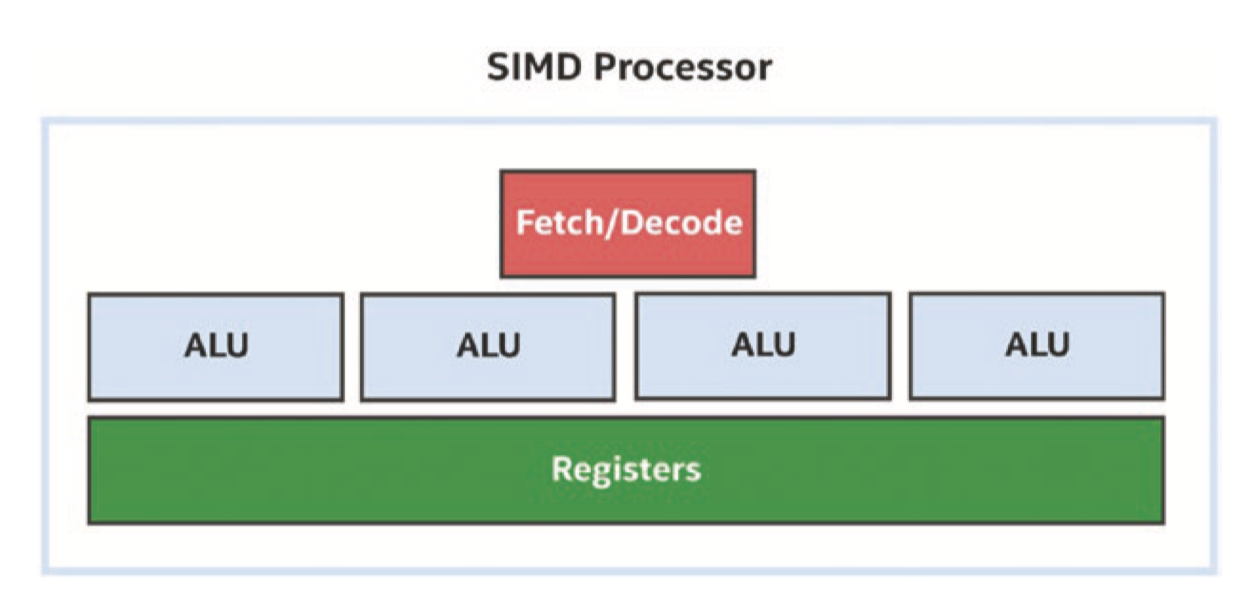
\includegraphics[width=0.9\textwidth]{figs/F15.8.png}
	\caption{\textit{四宽 SIMD 处理器:四个 ALU 共享获取/解码逻辑 }}
\end{figure}

由单个指令同时处理的数据元素的数量有时被称为指令或执行指令的处理器的SIMD宽度。 
在图 15-8 中,四个 ALU 共享相同的控制逻辑,因此可以将其描述为四宽 SIMD 处理器。

GPU 处理器并不是唯一实现 SIMD 指令集的处理器。 
其他处理器类型也实现 SIMD 指令集,以提高处理大型数据集时的效率。 
GPU 处理器与其他处理器类型之间的主要区别在于,GPU 处理器依靠并行执行多个数据元素来实现良好的性能,
并且 GPU 处理器可以支持比其他处理器类型更宽的 SIMD 宽度。 
例如,GPU 处理器支持 16、32 或更多数据元素的 SIMD 宽度并不罕见。

\begin{remark}[编程模型:SPMD 和 SIMD]
尽管 GPU 处理器实现具有不同宽度的 SIMD 指令集,但这通常是一个实现细节,
并且对于在 GPU 处理器上执行数据并行Kernel的应用程序是透明的。
这是因为许多 GPU 编译器和运行时 APIs 实现单个程序、多个数据或 SPMD 编程模型,
其中 GPU 编译器和运行时 APIs 确定要使用 SIMD 指令流处理的最有效的数据元素组,而不是显式表示 SIMD 指令。
第 9 章的“Sub-Groups”部分探讨了数据元素分组对应用程序可见的情况。
\end{remark}

\begin{figure}[H]
	\centering
	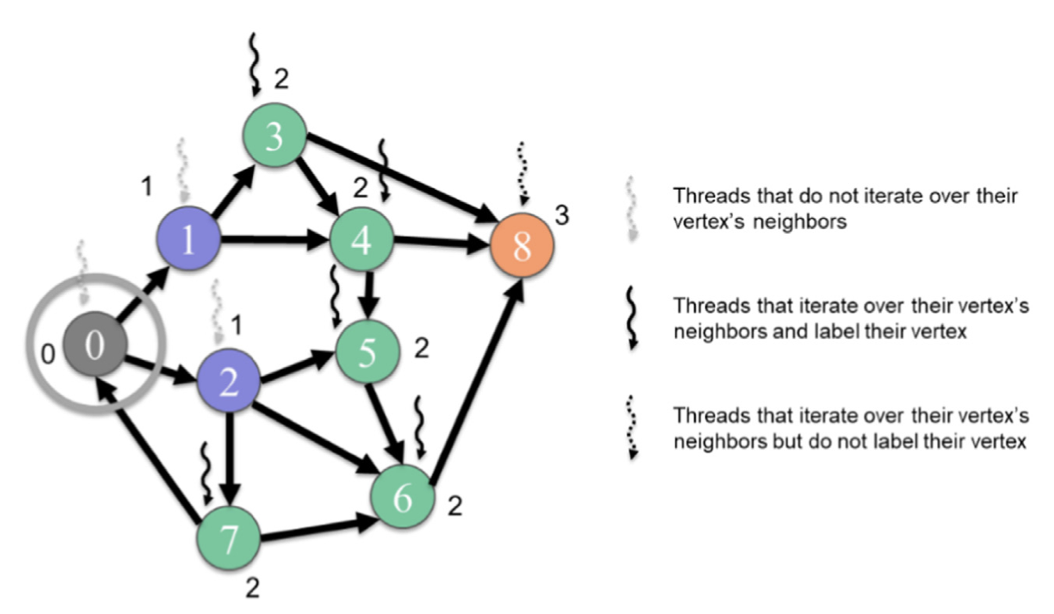
\includegraphics[width=0.9\textwidth]{figs/F15.9.png}
	\caption{\textit{在 SIMD 处理器上执行某种并行Kernel }}
\end{figure}

在图 15-9 中,我们扩展了每个执行资源以支持四宽 SIMD,从而允许我们并行处理四倍数量的矩阵行。

使用并行处理多个数据元素的 SIMD 指令是图 15-5 
和 15-7 中并行矩阵乘法Kernel的性能能够扩展到超出处理器数量的方法之一。 
在许多情况下,SIMD 指令的使用还提供了自然的局部性优势,包括通过在同一处理器上执行连续数据元素来进行矩阵乘法。

\begin{remark}
	Kernel受益于处理器之间的并行性和处理器内的并行性!
\end{remark}

\paragraph{预测和掩蔽}

只要所有数据元素通过Kernel中的条件代码采用相同的路径,在多个数据元素之间共享指令流就可以很好地工作。 
当数据元素通过条件代码采取不同的路径时,控制流被称为发散。 
当控制流在 SIMD 指令流中出现分歧时,通常会执行两个控制流路径,并屏蔽或预测某些通道。 
这确保了正确的行为,但正确性是以性能为代价的,因为被屏蔽的通道不会执行有用的工作。

\begin{figure}[H]
	\centering
	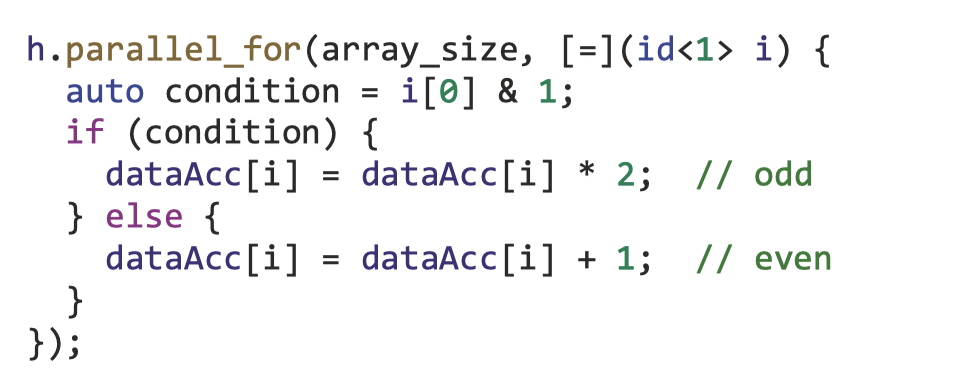
\includegraphics[width=0.9\textwidth]{figs/F15.10.png}
	\caption{\textit{具有发散控制流的Kernel }}
\end{figure}

为了展示预测和屏蔽的工作原理,请考虑图 15-10 中的Kernel,
它将每个具有“奇数”索引的数据元素乘以 2,并将每个具有“偶数”索引的数据元素递增 1。

假设我们在图 15-8 所示的四宽 SIMD 处理器上执行此Kernel,并且我们在一个 SIMD 指令流中执行前四个数据元素,
在不同的 SIMD 指令流中执行接下来的四个数据元素,等等 在。 
图 15-11 显示了可以屏蔽通道和预测执行以使用发散控制流正确执行该Kernel的方法之一。

\begin{figure}[H]
	\centering
	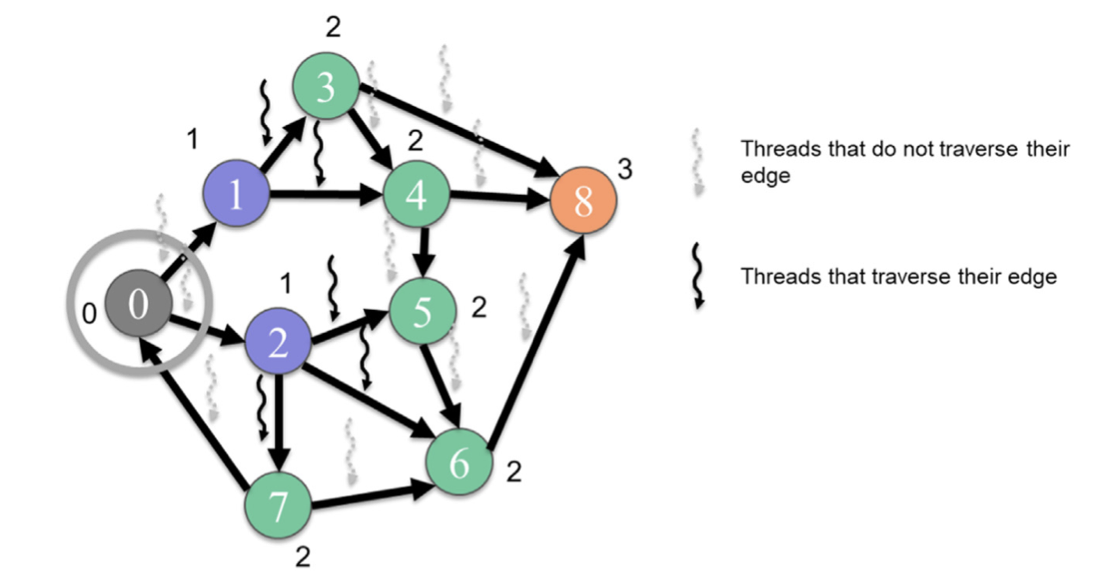
\includegraphics[width=0.9\textwidth]{figs/F15.11.png}
	\caption{\textit{发散Kernel的可能通道掩码 }}
\end{figure}

\paragraph{SIMD效率}

SIMD 效率衡量 SIMD 指令流与等效标量指令流相比的性能。 
在图15-11中,由于控制流将通道分为两个相等的组,因此发散控制流中的每条指令的执行效率只有一半。

在最坏的情况下,对于高度发散的Kernel,效率可能会降低处理器 SIMD 宽度的一个因子。

所有实现 SIMD 指令集的处理器都将遭受影响 SIMD 效率的发散性惩罚,
但由于 GPU 处理器通常支持比其他处理器类型更宽的 SIMD 宽度,
因此在优化时重构算法以最小化发散控制流并最大化收敛执行可能特别有益 GPU 的Kernel。 
这并不总是可能的,但作为示例,
选择沿具有更收敛执行的维度进行并行化可能比沿具有高度发散的执行的不同维度进行并行化表现得更好。

\paragraph{SIMD 效率和项目组}

到目前为止,本章中的所有Kernel都是基本数据并行Kernel,它们没有指定执行范围内的任何项目分组,
这使得实现可以自由地选择设备的最佳分组。 例如,具有较宽 SIMD 宽度的设备可能更喜欢较大的分组,
但具有较窄 SIMD 宽度的设备可能适合较小的分组。

当Kernel是具有显式Work-Items分组的 ND 范围Kernel时,应注意选择能够最大化 SIMD 效率的 ND 范围Work-Groups大小。 
当Work-Groups大小不能被处理器的 SIMD 宽度整除时,部分Work-Groups可能会在Kernel的整个持续时间内禁用通道来执行。 
针对 preferred\_work\_group\_size\_multiple 的设备特定Kernel查询可用于选择有效的 Work-Groups大小。 
有关如何查询设备属性的详细信息,请参阅第 12 章。

\begin{figure}[H]
	\centering
	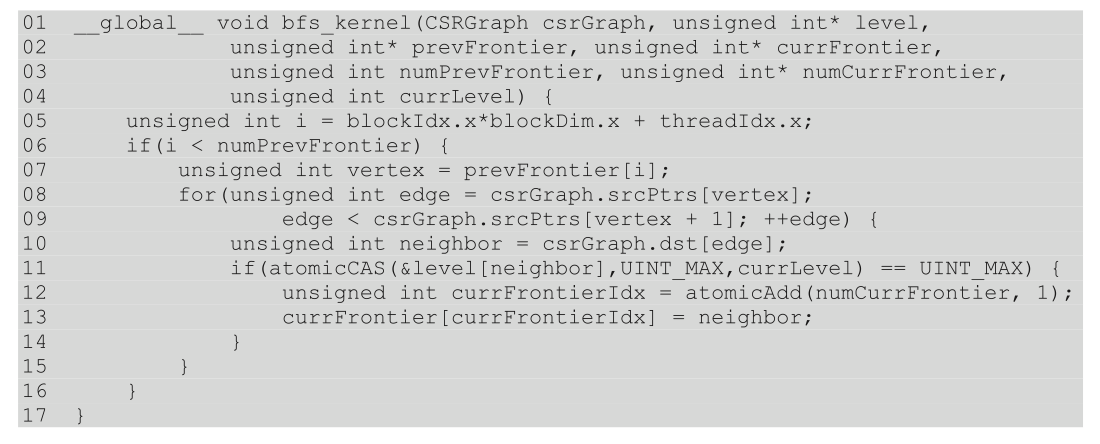
\includegraphics[width=0.9\textwidth]{figs/F15.12.png}
	\caption{\textit{低效的单项、有点平行的矩阵乘法 }}
\end{figure}

选择由单个Work-Items组成的Work-Groups大小可能会表现得很差,
因为许多 GPU 将通过屏蔽除一个通道之外的所有 SIMD 通道来实现单Work-Items 的 Work-Groups。 
例如,图 15-12 中的Kernel的性能可能会比图 15-5 中非常相似的Kernel差很多,
尽管两者之间唯一的显着区别是从基本数据并行Kernel到低效的单并行Kernel的变化。 
Work-Items ND 范围Kernel (nd\_range<1>{M, 1})。

\subsubsection{切换工作以隐藏延迟}
许多 GPU 使用另一种技术来简化控制逻辑、最大化执行资源并提高性能:许多 GPU 允许多个指令流同时驻留在处理器上,
而不是在处理器上执行单个指令流。

在处理器上驻留多个指令流是有益的,因为它使每个处理器都可以选择要执行的工作。 
如果一个指令流正在执行长延迟操作,例如从内存读取,则处理器可以切换到准备运行的不同指令流,而不是等待操作完成。 
有了足够的指令流,当处理器切换回原始指令流时,长延迟操作可能已经完成,而无需处理器等待。

\begin{figure}[H]
	\centering
	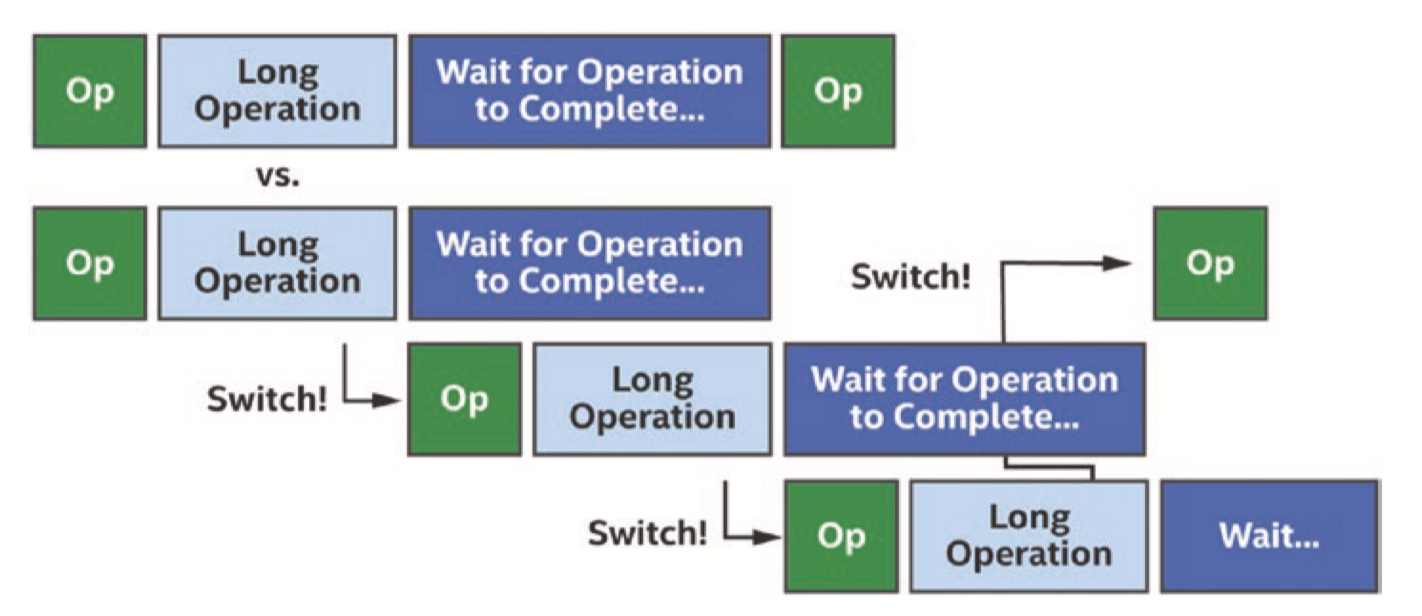
\includegraphics[width=0.9\textwidth]{figs/F15.13.png}
	\caption{\textit{切换指令流以隐藏延迟 }}
\end{figure}

图 15-13 显示了处理器如何使用多个同时指令流来隐藏延迟并提高性能。 
尽管第一个指令流在多个流中执行的时间稍长,但通过切换到其他指令流,
处理器能够找到准备执行的工作,而无需空闲地等待长时间操作完成。

GPU 分析工具可以使用诸如占用率之类的术语来描述 GPU 处理器当前正在执行的指令流数量与理论指令流总数的关系。

低占用率并不一定意味着低性能,因为少量指令流可能会使处理器保持忙碌。 
同样,高占用率并不一定意味着高性能,因为如果所有指令流都执行低效、长延迟的操作,GPU 处理器可能仍然需要等待。 
不过,在其他条件相同的情况下,增加占用率可以最大限度地提高 GPU 处理器隐藏延迟的能力,并且通常会提高性能。 
增加占用率是使用图 15-7 中更加并行的Kernel可以提高性能的另一个原因。

这种在多个指令流之间切换以隐藏延迟的技术特别适合 GPU 和数据并行处理。 
回想一下图 15-2,GPU 处理器通常比其他处理器类型更简单,因此缺乏复杂的延迟隐藏功能。 
这使得 GPU 处理器更容易受到延迟问题的影响,但由于数据并行编程涉及处理大量数据,GPU 处理器通常有大量指令流要执行!

\subsection{将Kernel卸载到 GPU}
\begin{figure}[H]
	\centering
	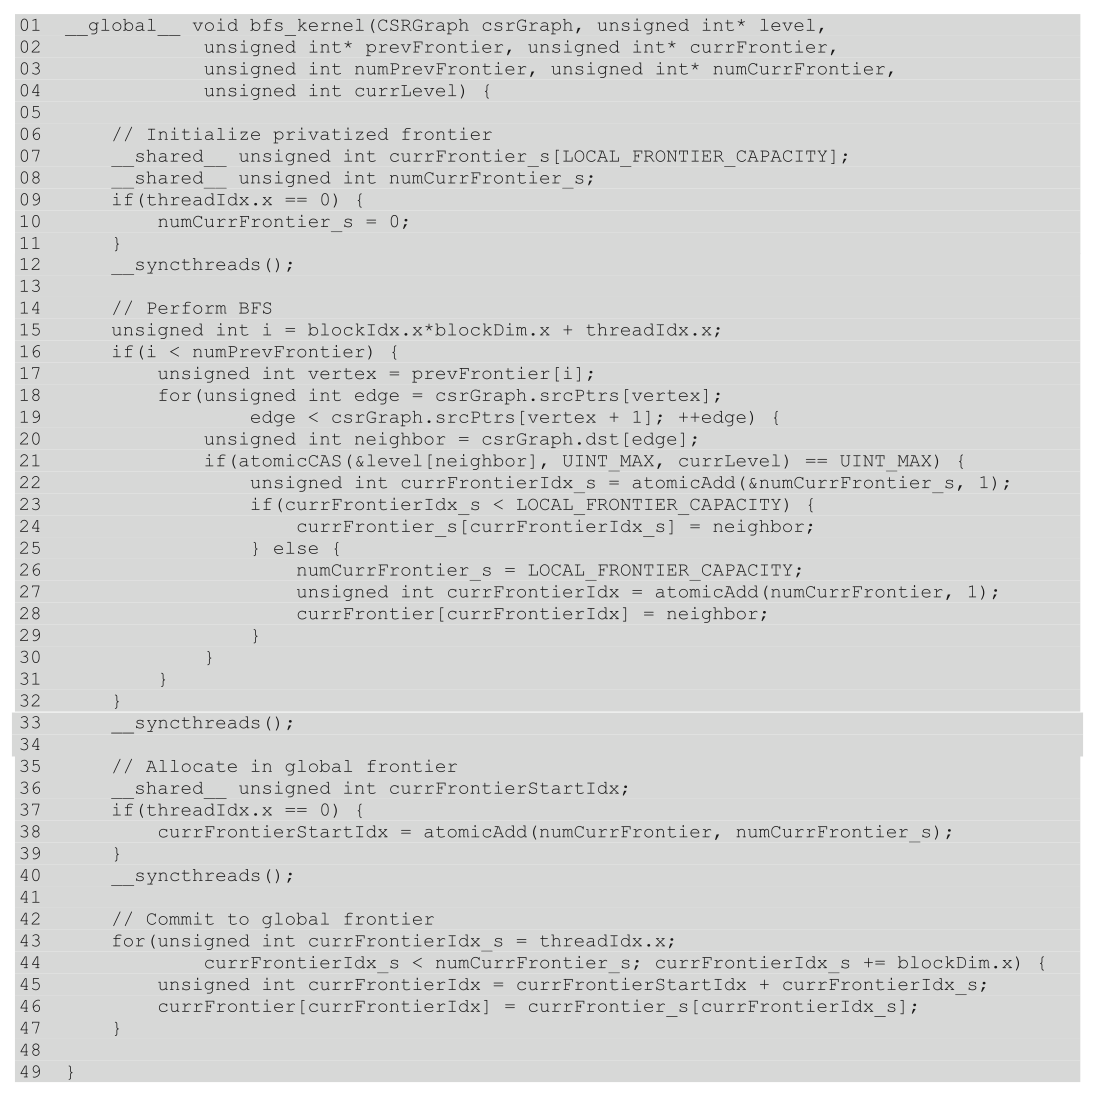
\includegraphics[width=0.9\textwidth]{figs/F15.14.png}
	\caption{\textit{将并行Kernel卸载到 GPU(简化)}}
\end{figure}

本节介绍应用程序、SYCL 运行时库和 GPU 软件驱动程序如何协同工作以在 GPU 硬件上卸载Kernel。 
图 15-14 中的图表显示了具有这些抽象层的典型软件堆栈。 
在许多情况下,这些层的存在对于应用程序来说是透明的,但在调试或分析应用程序时理解并考虑它们非常重要。

\subsubsection{SYCL 运行时库}
SYCL 运行时库是 SYCL 应用程序与之交互的主要软件库。 
运行时库负责实现队列、Buffer和访问器等类以及这些类的成员函数。 
运行时库的某些部分可能位于头文件中,因此可以直接编译到应用程序可执行文件中。 
运行时库的其他部分作为库函数实现,作为应用程序构建过程的一部分与应用程序可执行文件链接。 
运行时库通常不是特定于设备的,并且同一运行时库可以协调卸载到 CPU、GPU、FPGA 或其他设备。

\subsubsection{GPU 软件驱动程序}
尽管理论上 SYCL 运行时库可以直接卸载到 GPU,
但实际上,大多数 SYCL 运行时库与 GPU 软件驱动程序连接以将工作提交到 GPU。

GPU 软件驱动程序通常是 API 的实现,例如 OpenCL、零级或 CUDA。 
大多数GPU软件驱动程序都是在SYCL运行时调用的用户模式驱动程序库中实现的,
并且用户模式驱动程序可以调用操作系统或Kernel模式驱动程序来执行系统级任务,例如分配内存 或向设备提交工作。 
用户模式驱动程序还可以调用其他用户模式库; 
例如,GPU驱动程序可以调用GPU编译器来将Kernel从中间表示及时编译为GPU ISA(指令集架构)。 
这些软件模块以及它们之间的交互如图15-15所示。

\begin{figure}[H]
	\centering
	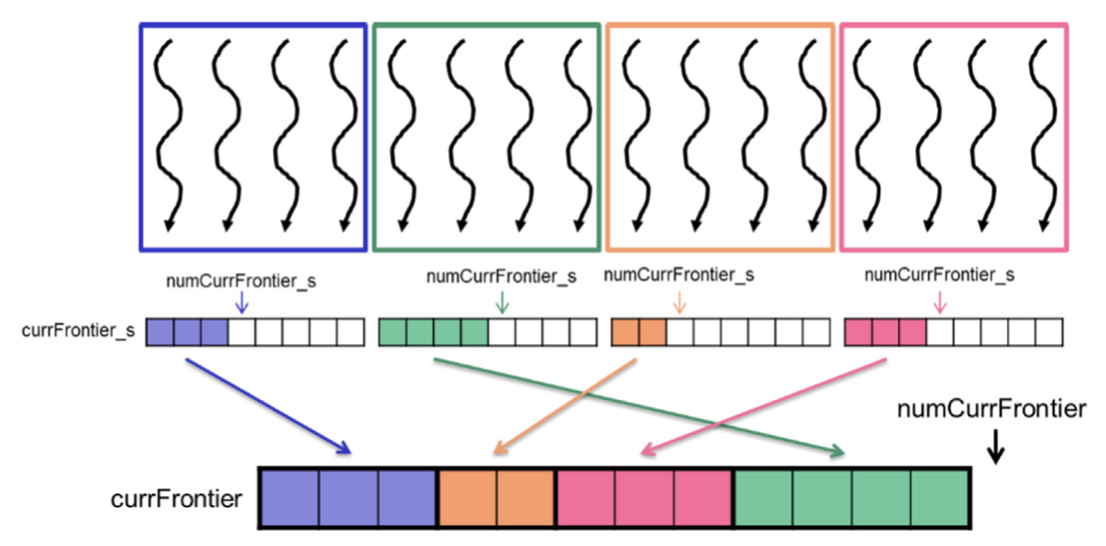
\includegraphics[width=0.9\textwidth]{figs/F15.15.png}
	\caption{\textit{典型的 GPU 软件驱动程序模块}}
\end{figure}

\subsubsection{GPU硬件}
当运行时库或 GPU 软件用户模式驱动程序被明确请求提交工作时,
或者当 GPU 软件试探性地确定工作应该开始时,它通常会通过操作系统或Kernel模式驱动程序调用来开始执行工作 GPU。 
在某些情况下,GPU 软件用户模式驱动程序可能会直接向 GPU 提交工作,
但这种情况不太常见,并且可能并非所有设备或操作系统都支持。

当 GPU 上执行的工作结果被主机处理器或另一个加速器消耗时,GPU 必须发出信号以指示工作已完成。 
工作完成涉及的步骤与工作提交的步骤非常相似,
执行方向相反:GPU 可能会向操作系统或Kernel模式驱动程序发出信号,表明其已完成执行,然后通知用户模式驱动程序,
最后 运行时库将通过 GPU 软件 API 调用观察到工作已完成。

每个步骤都会引入延迟,并且在许多情况下,运行时库和 GPU 软件会在较低延迟和较高吞吐量之间进行权衡。 
例如,更频繁地向 GPU 提交工作可能会减少延迟,但频繁提交也可能会因每次提交的开销而降低吞吐量。 
收集大批量的工作会增加延迟,但可以分摊更多工作的提交开销,并引入更多并行执行的机会。 
运行时和驱动程序经过调整以做出正确的权衡,并且通常会做得很好,
但是如果我们怀疑驱动程序启发式提交工作效率低下,
我们应该查阅文档以查看是否有方法使用 API 覆盖默认驱动程序行为 -特定的甚至特定于实现的机制。 
第 20 章中描述的直接与 API 后端交互的技术对于调整 GPU 提交策略非常有用。

\subsubsection{当心卸载成本!}
尽管 SYCL 实现和 GPU 供应商不断创新和优化,以降低将工作卸载到 GPU 的成本,
但在 GPU 上开始工作以及在主机或其他设备上观察结果时总会产生开销。 
选择在何处执行算法时,请考虑在设备上执行算法的好处以及将算法及其所需的任何数据移动到设备的成本。 
在某些情况下,使用主机处理器执行并行操作可能是最有效的,
或者在 GPU 上低效地执行算法的串行部分,以避免将算法从一个处理器移动到另一个处理器的开销。

\begin{remark}
	考虑我们算法的整体性能 - 在一台设备上低效地执行部分算法可能比将执行转移到另一台设备更有效!
\end{remark}

\paragraph{与设备内存之间的传输}

\begin{figure}[H]
	\centering
	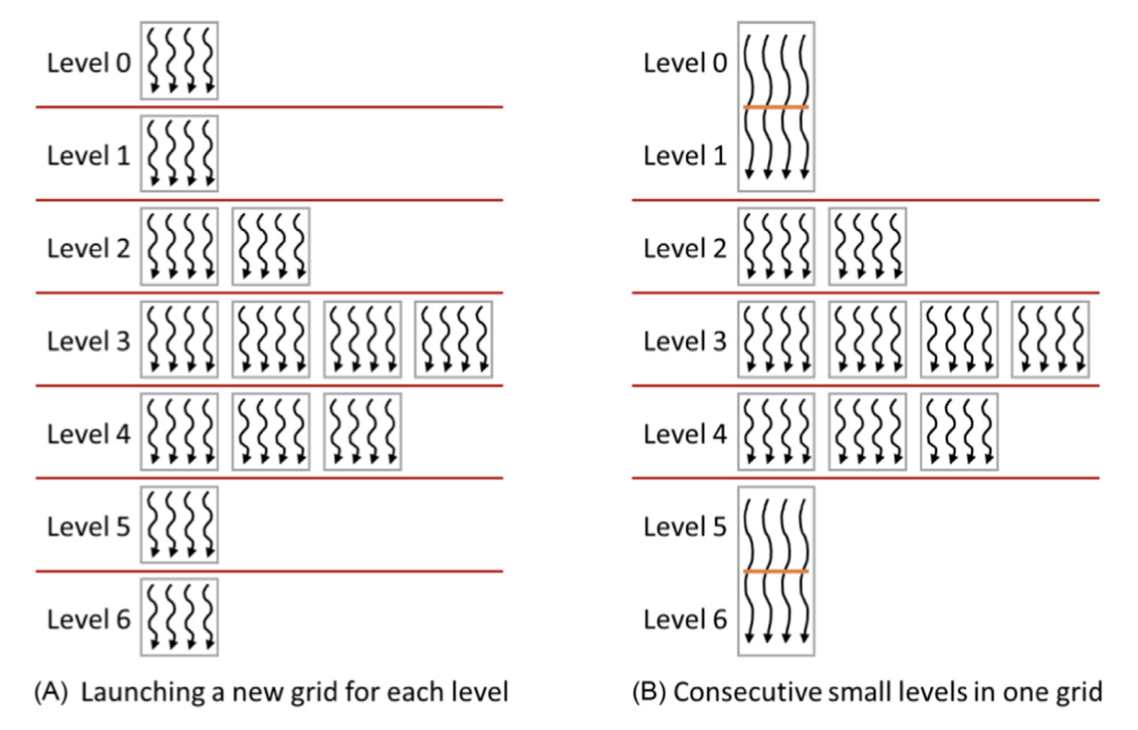
\includegraphics[width=0.9\textwidth]{figs/F15.16.png}
	\caption{\textit{设备内存、远程内存和主机内存之间的典型差异}}
\end{figure}

在具有专用内存的 GPU 上,请特别注意专用 GPU 内存与主机或其他设备上的内存之间的传输成本。 
图 15-16 显示了系统中不同内存类型之间的典型内存带宽差异。

回想一下第 3 章,GPU 更喜欢在专用设备内存上运行,这样速度可以快一个数量级或更多,
而不是在主机内存或其他设备的内存上运行。 
尽管对专用设备内存的访问比对远程内存或系统内存的访问要快得多,
但如果数据尚未位于专用设备内存中,则必须对其进行复制或迁移。

只要数据会被频繁访问,将其移至专用设备内存中就是有益的,
特别是当 GPU 执行资源忙于处理另一项任务时可以异步执行传输时。 
然而,当数据访问不频繁或不可预测时,即使每次访问成本较高,最好还是节省传输成本并远程或在系统内存中对数据进行操作。 
第 6 章介绍了控制内存分配位置的方法以及将数据复制和预取到专用设备内存的不同技术。 
这些技术在优化 GPU 程序执行时非常重要。

\subsection{GPU Kernel最佳实践}
前面的部分描述了传递给parallel\_for 的调度参数如何影响Kernel分配给GPU 处理器资源的方式
以及在GPU 上执行Kernel所涉及的软件层和开销。 本节介绍Kernel在 GPU 上执行时的最佳实践。

从广义上讲,Kernel要么是内存限制的,这意味着它们的性能受到 GPU 上执行资源的数据读写操作的限制,
要么是计算限制,这意味着它们的性能受到 GPU 上执行资源的限制 。 
为 GPU(以及许多其他处理器)优化Kernel时,第一步是确定我们的Kernel是内存限制型还是计算限制型,
因为经常改进内存限制型Kernel的技术不会使计算限制型Kernel受益 反之亦然。 
GPU 供应商通常会提供分析工具来帮助做出这一决定。

\begin{remark}
	需要不同的优化技术,这取决于我们的Kernel是内存受限还是计算受限!
\end{remark}

由于 GPU 往往具有许多处理器和较宽的 SIMD 宽度,因此Kernel往往更多地受到内存限制而不是计算限制。 
如果我们不确定从哪里开始,检查Kernel如何访问内存是一个很好的第一步。

\subsubsection{访问全局内存}
有效访问全局内存对于优化应用程序性能至关重要,因为Work-Items或Work-Groups操作的几乎所有数据都源自全局内存。 
如果Kernel对全局内存的操作效率低下,它几乎总是会表现得很差。 
尽管 GPU 通常包含用于读取和写入内存中任意位置的专用硬件收集和分散单元,
但对全局内存的访问性能通常由数据访问的局部性驱动。 
如果Work-Groups中的一个Work-Items正在访问存储器中与Work-Groups中的另一Work-Items所访问的元素相邻的元素,
则全局存储器访问性能可能良好。 
如果Work-Groups中的Work-Items改为跨步或随机访问内存,则全局内存访问性能可能会更差。 
一些 GPU 文档将附近内存访问的操作描述为合并内存访问。

回想一下,对于图 15-5 中的稍微并行的矩阵乘法Kernel,我们可以选择是否并行处理结果矩阵的行或列,
并且我们选择并行操作结果矩阵的行。 
事实证明这是一个糟糕的选择:如果 id 等于 m 的一个Work-Items与 id 等于 m-1 或 m+1 的相邻Work-Items分组,
则用于访问矩阵 B 的索引对于每个Work-Items都是相同的 Work-Items,
但用于访问矩阵 A 的索引相差 K,这意味着访问是高度跨步的。 
矩阵 A 的访问模式如图 15-17 所示。

\begin{figure}[H]
	\centering
	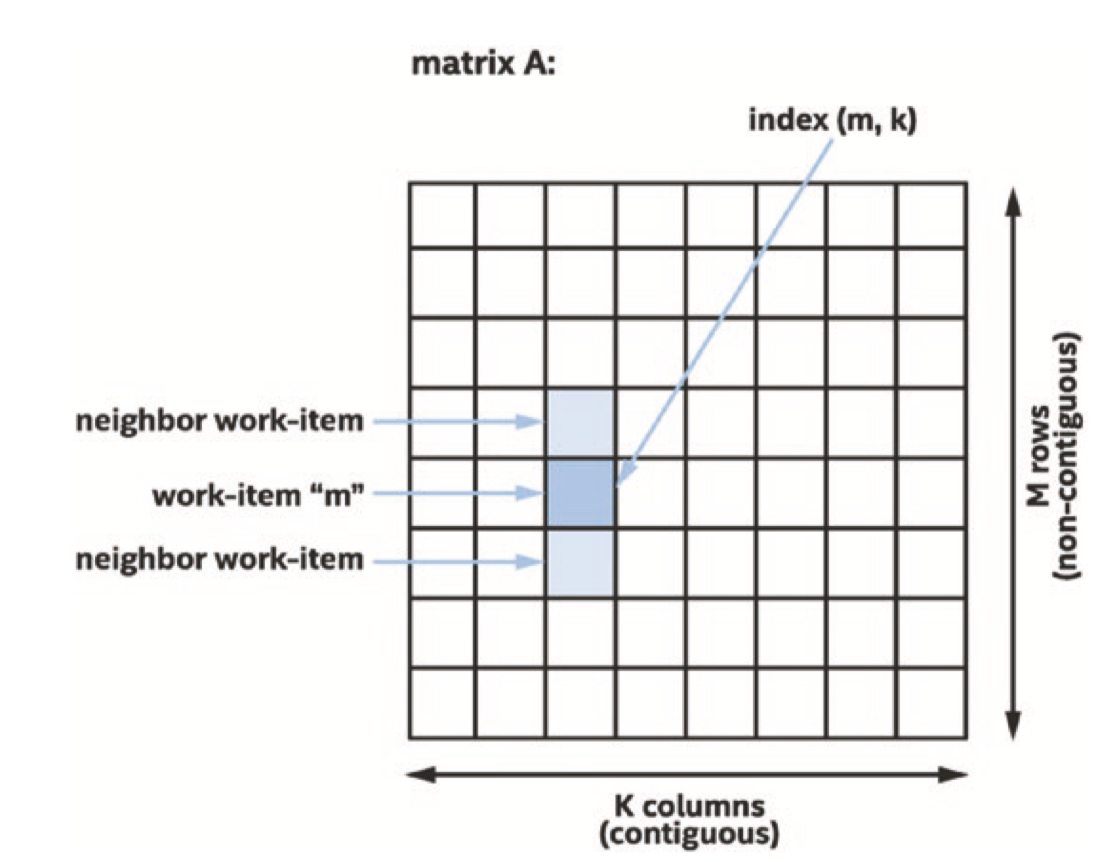
\includegraphics[width=0.9\textwidth]{figs/F15.17.png}
	\caption{\textit{对矩阵A的访问非常缓慢且效率低下}}
\end{figure}

相反,如果我们选择并行处理结果矩阵的列,则访问模式具有更好的局部性。 
图15-18中的Kernel在结构上与图15-5中的Kernel非常相似,
唯一的区别是图15-18中的每个Work-Items对结果矩阵的列进行操作,而不是对结果矩阵的行进行操作 。

\begin{figure}[H]
	\centering
	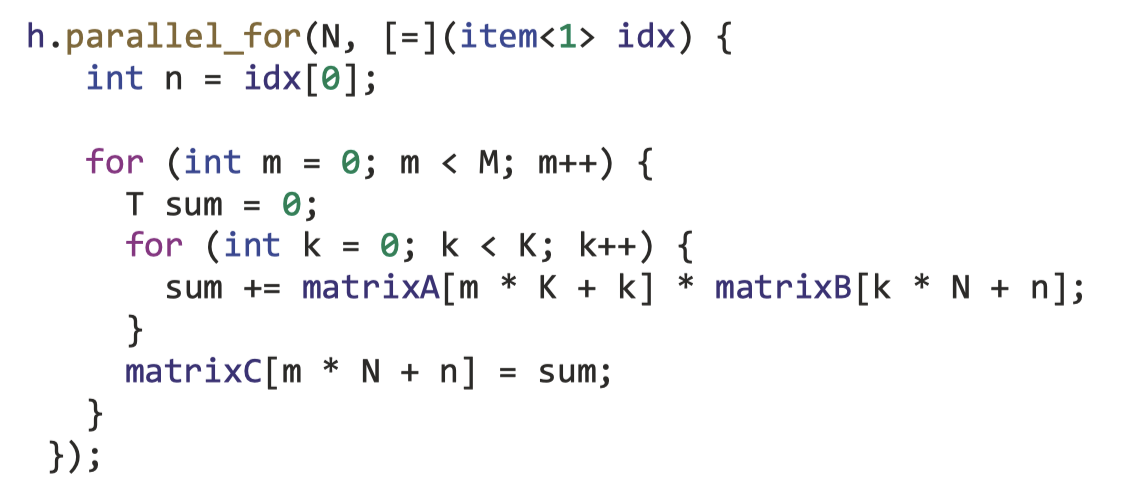
\includegraphics[width=0.9\textwidth]{figs/F15.18.png}
	\caption{\textit{并行计算结果矩阵的列,而不是行}}
\end{figure}

尽管这两个Kernel在结构上非常相似,但在许多 GPU 上,对数据列进行操作的Kernel将显着优于对数据行进行操作的Kernel,
这纯粹是由于更高效的内存访问:如果一个Work-Items的 id 相等 to n 与 id 等于 n-1 或 n+1 的相邻Work-Items分组,
用于访问矩阵 A 的索引现在对于每个Work-Items都是相同的,并且用于访问矩阵 B 的索引是连续的。 
矩阵 B 的访问模式如图 15-19 所示。

\begin{figure}[H]
	\centering
	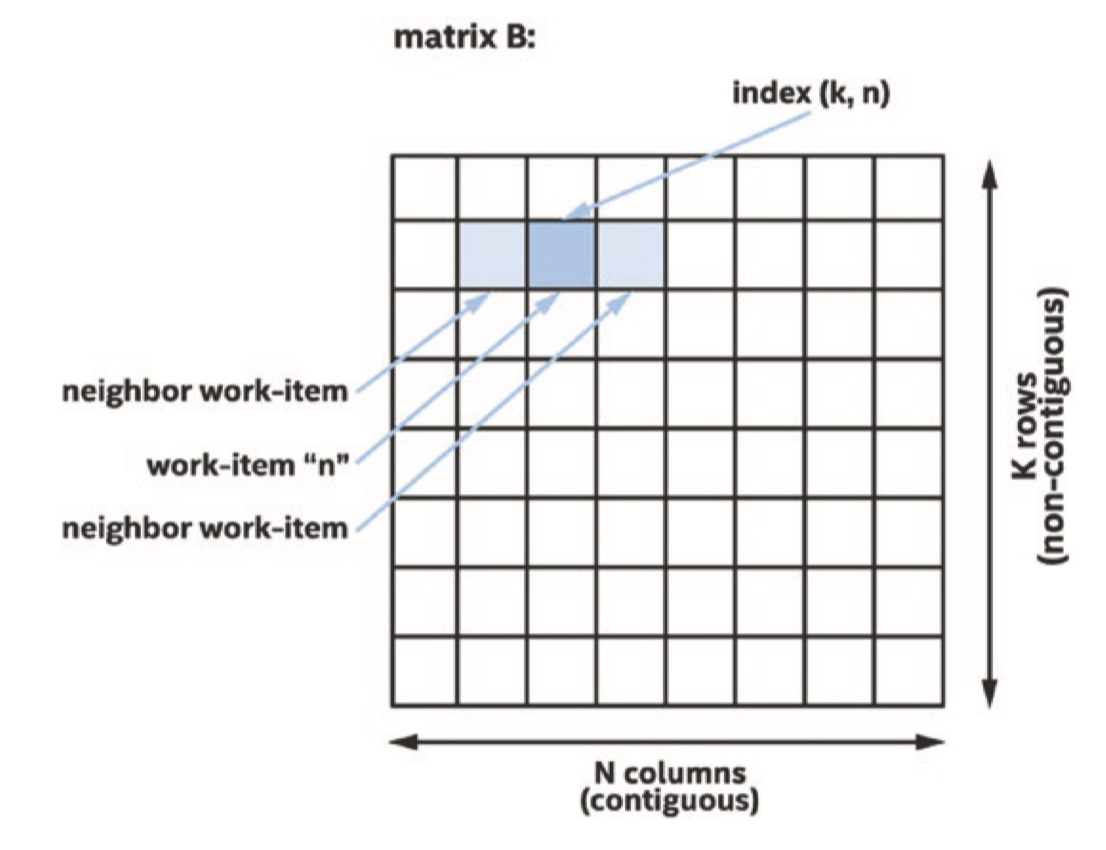
\includegraphics[width=0.9\textwidth]{figs/F15.19.png}
	\caption{\textit{对 matrixB 的访问是连续且高效的}}
\end{figure}

对连续数据的访问通常非常有效。 一个好的经验法则是,一组Work-Items对全局内存的访问性能是所访问的 GPU 缓存行数量的函数。 
如果所有访问都在单个高速缓存行内,则访问将以峰值性能执行。 
如果访问需要两个高速缓存行,例如通过访问每个其他元素或从高速缓存未对齐的地址开始,则访问可能会以一半的性能运行。 
当组中的每个Work-Items访问唯一的高速缓存行时,例如跨步或随机访问,访问可能会以最低性能运行。

\begin{remark}[分析Kernel变体]
对于矩阵乘法,选择沿一个维度并行化显然会导致更有效的内存访问,但对于其他Kernel,选择可能并不那么明显。
对于实现最佳性能很重要的Kernel,如果不清楚要并行化哪个维度,
有时值得开发和分析沿每个维度并行化的不同Kernel变体,以了解什么更适合设备和数据集。
\end{remark}

\subsubsection{访问Work-Groups本地内存}
在上一节中,我们描述了对全局内存的访问如何受益于局部性,以最大限度地提高缓存性能。 
正如我们所看到的,在某些情况下,我们可以设计算法来有效地访问内存,例如选择在一个维度而不是另一个维度进行并行化。 
然而,这种技术并非在所有情况下都可行。 本节介绍如何使用Work-Groups本地内存来有效支持更多内存访问模式。

回想一下第 9 章,Work-Groups中的Work-Items可以通过Work-Groups本地内存进行通信
并使用Work-Groups障碍进行同步来合作解决问题。 
该技术对于 GPU 特别有利,因为典型的 GPU 具有专门的硬件来实现屏障和Work-Groups本地内存。 
不同的 GPU 供应商和不同的产品可能会以不同的方式实现Work-Groups本地内存,
但与全局内存相比,Work-Groups本地内存通常有两个好处:本地内存可以支持比全局内存访问更高的带宽和更低的延迟,
即使全局内存 访问会命中缓存,本地内存通常分为不同的内存区域,称为存储体。 
只要组中的每个Work-Items访问不同的存储体,本地内存访问就会以最佳性能执行。 
与全局内存相比,分组访问允许本地内存以峰值性能支持更多的访问模式。

许多GPU供应商会将连续的本地内存地址分配给不同的bank。 这确保了连续的内存访问始终以最佳性能运行,无论起始地址如何。 
然而,当内存访问跨步时,组中的某些Work-Items可能会访问分配给同一存储体的内存地址。 
发生这种情况时,会被视为存储体冲突并导致串行访问和性能降低。

\begin{remark}
为了实现最大的全局内存性能,请最大程度地减少访问的缓存行数。

为了获得最大的本地内存性能,请最大限度地减少 bank 冲突的数量!
\end{remark}

\begin{figure}[H]
	\centering
	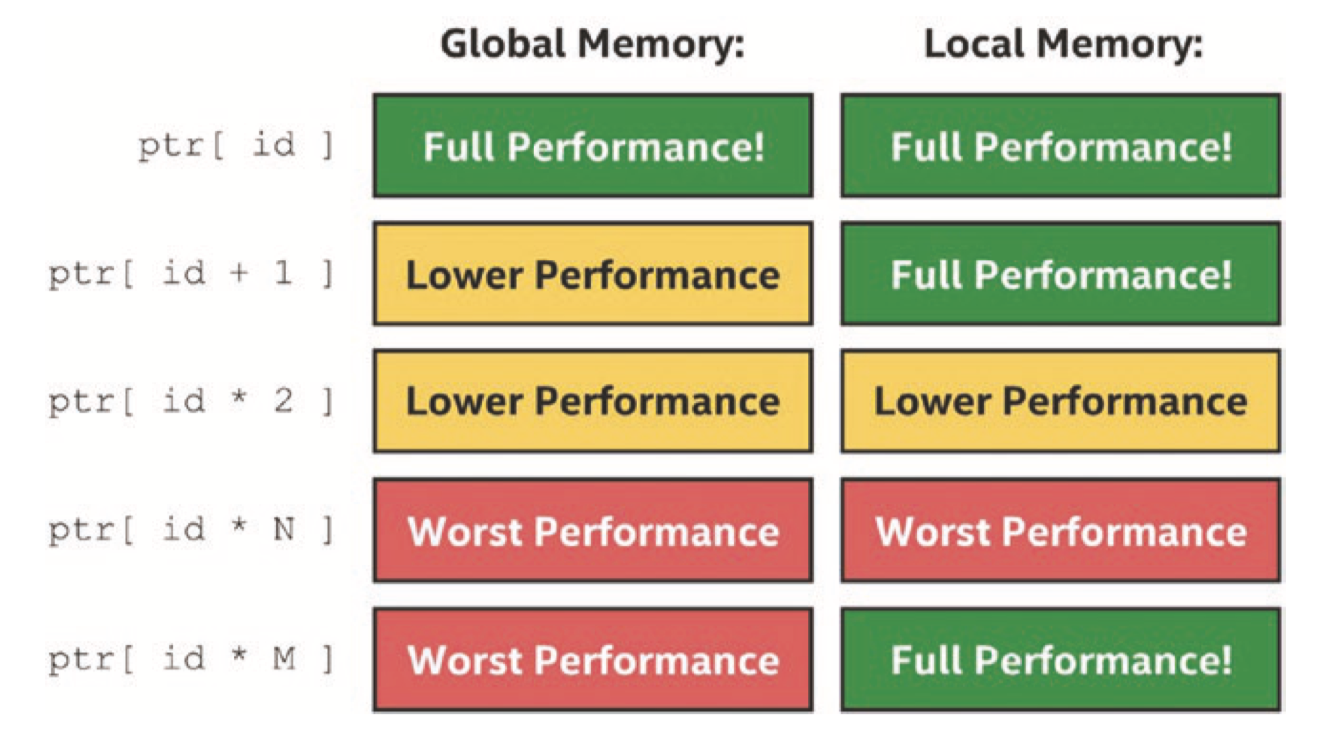
\includegraphics[width=0.9\textwidth]{figs/F15.20.png}
	\caption{\textit{不同访问模式、全局和本地内存的可能性能}}
\end{figure}

全局内存和本地内存的访问模式和预期性能摘要如图 15-20 所示。 
假设当 ptr 指向全局内存时,指针与 GPU 缓存行的大小对齐。 
通过从缓存对齐地址开始连续访问内存,可以实现访问全局内存时的最佳性能。 
访问未对齐的地址可能会降低全局内存性能,因为该访问可能需要访问额外的缓存行。 
由于访问未对齐的本地地址不会导致额外的存储体冲突,因此本地内存性能保持不变。

跨步案例值得更详细地描述。 访问全局内存中的每个其他元素需要访问更多的缓存行,并且可能会导致性能降低。 
访问本地内存中的所有其他元素可能会导致存储体冲突和性能降低,但前提是存储体的数量可以被 2 整除。 
如果银行的数量是奇数,这种情况也将在全性能下运行。

当访问之间的步幅非常大时,每个Work-Items都会访问唯一的缓存行,从而导致性能最差。 
但对于本地内存,性能取决于步幅和存储体数量。 
当步长N等于Bank数时,每次访问都会导致Bank冲突,并且所有访问都是串行的,导致性能最差。 
然而,如果步长 M 和存储体数量没有共同因素,则访问将以全部性能运行。 
因此,许多优化的 GPU Kernel会在本地内存中填充数据结构,以选择减少或消除存储体冲突的步幅。

\subsubsection{通过Sub-Groups完全避免本地内存}
正如第 9 章所讨论的,Sub-Groups集体功能是在组中的Work-Items之间交换数据的另一种方法。 
对于许多 GPU 来说,Sub-Groups代表由单个指令流处理的Work-Items的集合。 
在这些情况下,Sub-Groups中的Work-Items可以廉价地交换数据并同步,而无需使用Work-Groups本地存储器。 
许多性能最佳的 GPU Kernel都使用Sub-Groups,因此对于昂贵的Kernel,
非常值得检查我们的算法是否可以重新表述为使用Sub-Groups集体函数。

\subsubsection{使用小数据类型优化计算}
本节介绍在消除或减少内存访问瓶颈后优化Kernel的技术。 
需要牢记的一个非常重要的观点是,GPU 传统上被设计用于在屏幕上绘制图片。 
尽管 GPU 的纯计算能力随着时间的推移不断发展和提高,但在某些领域,其图形传统仍然很明显。

例如,考虑对Kernel数据类型的支持。 许多 GPU 针对 32 位浮点运算进行了高度优化,因为这些运算在图形和游戏中很常见。 
对于可以处理较低精度的算法,许多 GPU 还支持较低精度的 16 位浮点类型,以牺牲精度来换取更快的处理速度。 
相反,虽然许多 GPU 确实支持 64 位双精度浮点运算,但额外的精度是有代价的,
而且 32 位运算的性能通常比 64 位等效运算要好得多。

对于整数数据类型也是如此,其中 32 位整数数据类型的性能通常优于 64 位整数数据类型,而 16 位整数的性能可能甚至更好。 
如果我们可以构建我们的计算以使用较小的整数,我们的Kernel可能会执行得更快。 
需要特别注意的一个领域是寻址操作,它通常对 64 位 size\_t 数据类型进行操作,
但有时可以重新排列以使用 32 位数据类型执行大部分计算。 
在某些本地内存情况下,16 位索引就足够了,因为大多数本地内存分配都很小。

\subsubsection{优化数学函数}
Kernel可能会为了性能而牺牲准确性的另一个领域涉及 SYCL 内置函数。 
SYCL 包含一组丰富的数学函数,在一系列输入中具有明确定义的精度。 
大多数 GPU 本身并不支持这些功能,而是使用一长串其他指令来实现它们。 
尽管数学函数实现通常针对 GPU 进行了很好的优化,但如果我们的应用程序可以容忍较低的精度,
我们应该考虑采用精度较低但性能较高的不同实现。 有关 SYCL 内置函数的更多信息,请参阅第 18 章。

对于常用的数学函数,SYCL 库包括具有降低的或实现定义的精度要求的快速或本机函数变体。 
对于某些 GPU,这些函数可能比其精确的等效函数快一个数量级,因此如果它们对算法具有足够的精度,则非常值得考虑。 
例如,许多图像后处理算法具有明确定义的输入,并且可以容忍较低的精度,因此是使用快速或本机数学函数的良好候选者。

\subsubsection{特化功能和扩展}
优化 GPU Kernel时的最后一个考虑因素是许多 GPU 中常见的专用指令。 
举一个例子,几乎所有 GPU 都支持 mad 或 fma 乘加指令,该指令在单个时钟中执行两个操作。 
GPU 编译器通常非常擅长识别和优化单个乘法和加法以使用单个指令,但 SYCL 还包括可以显式调用的 mad 和 fma 函数。 
当然,如果我们希望 GPU 编译器为我们优化乘法和加法,我们应该确保我们不会通过禁用浮点收缩来阻止优化!

其他专用 GPU 指令可能只能通过编译器优化、SYCL 语言扩展或直接与低级 GPU 后端交互来获得。 
例如,某些 GPU 支持专门的点积累加指令,编译器将尝试识别并优化该指令,或者可以直接调用该指令。 
有关如何查询 GPU 实现支持的扩展的更多信息,请参阅第 12 章,有关后端互操作性的信息,请参阅第 20 章。

\begin{remark}
	如果算法可以容忍较低的精度,我们可以使用更小的数据类型或更低精度的数学函数来提高性能!
\end{remark}

\subsection{总结}
在本章中,我们首先描述典型 GPU 的工作原理以及 GPU 与传统 CPU 的不同之处。 
我们描述了如何通过将加速单个指令流的处理器功能换成额外的处理器来针对大量数据进行优化。

我们描述了 GPU 如何使用宽 SIMD 指令并行处理多个数据元素,
以及 GPU 如何使用预测和掩码来使用 SIMD 指令执行具有复杂流程控制的Kernel。 
我们讨论了预测和掩码如何降低 SIMD 效率并降低高度发散的Kernel的性能,
以及选择沿一个维度与另一维度并行化如何减少 SIMD 发散。

由于 GPU 拥有如此多的处理资源,我们讨论了为 GPU 提供足够的工作以保持高占用率的重要性。 
我们还描述了 GPU 如何使用指令流来隐藏延迟,这使得为 GPU 提供大量执行工作变得更加重要。

接下来,我们讨论了将Kernel卸载到 GPU 所涉及的软件和硬件层以及卸载的成本。 
我们讨论了在单个设备上执行算法如何比将执行从一个设备转移到另一个设备更有效。

最后,我们描述了Kernel在 GPU 上执行时的最佳实践。 
我们描述了有多少Kernel从内存限制开始,以及如何有效地访问全局内存和本地内存,
或者如何通过使用Sub-Groups操作完全避免本地内存。 
当Kernel受计算限制时,我们描述了如何通过以较低精度换取更高性能或使用自定义 GPU 扩展来访问专用指令来优化计算。

\subsubsection{了解更多信息}
关于 GPU 编程还有很多东西需要学习,本章只是触及了表面!

GPU 规范和白皮书是了解有关特定 GPU 和 GPU 架构的更多信息的好方法。 
许多 GPU 供应商提供了有关其 GPU 以及如何对其进行编程的非常详细的信息。

在撰写本文时,有关主要 GPU 的相关阅读可在 software.intel.com、devblogs.nvidia.com 和 amd.com 上找到。

一些 GPU 供应商拥有开源驱动程序或驱动程序组件。 
如果可用,检查或单步执行驱动程序代码可能会很有帮助,以了解哪些操作成本较高或应用程序中哪些地方可能存在开销。

本章完全关注通过Buffer访问器或统一共享内存对全局内存的传统访问,
但大多数 GPU 还包含一个固定函数纹理采样器,可以加速图像操作。 有关图像和采样器的更多信息,请参阅 SYCL 规范。